\section{Application Layer}



\subsection{Domain Name Space (DNS)}

\subsection{Dynamic Host Configuration Protocol (DHCP)}{
    { \begin{itemize}[noitemsep]
                \item Paketformat identisch zu BOOTP
                \item Dynamische Zuweisung von IP-Adressen
                \item PReserviert nur IP’s von aktiven Geräte

            \end{itemize}}

    \WhiteSpace
    {Ablauf (DHCP):
        \begin{itemize}[noitemsep]
            \item 1. Client sucht DHCP Server mittels Broadcast
            \item 2. DHCP Server antwortet (DHCP offer)
            \item 3. Der Client wählt einen Server und fordert eine
            \item 4. Der Server bestätigt mit einer Message, welche die endgültigen Parameter enthält
            \item 5. Vor Ablauf der Lease-Time erneuert der Client die
                  Adresse
        \end{itemize}
    }

}


\subsection{Network Address Translation (NAT)}
{
    NAT verletzt das Konzept der OSI-Layer, da eine Network-Funktion auf den Transport-Header
    zugreift. IP-Adresse und Portnummer werden dabei verändert.}
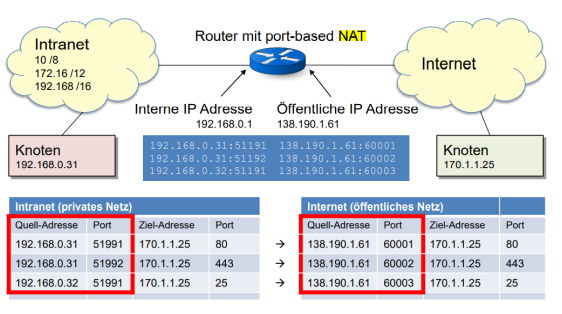
\includegraphics[scale=.45]{img/NAT.png}

\subsection{BOOTP}{
    \begin{itemize}[noitemsep]
        \item Manuelle Verwaltung
        \item Heimanwender sind überfordert
        \item Statische Adresszuordnung
    \end{itemize}

}



\subsection{Trivial File Transfer Protocol (TFTP)}
{Basiert auf UDP}
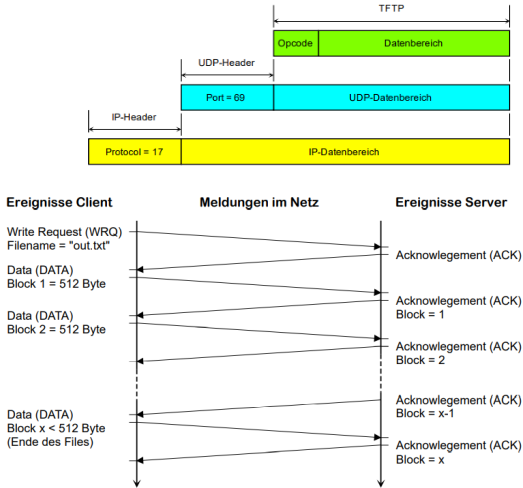
\includegraphics[scale=.5]{img/tftp.png}

\subsection{Simple Mail Transfer Protocol (SMTP)}


